%%=============================================================================
%% Methodologie
%%=============================================================================

\chapter{\IfLanguageName{dutch}{Methodologie}{Methodology}}
\label{ch:methodologie}

%% TODO: Hoe ben je te werk gegaan? Verdeel je onderzoek in grote fasen, en
%% licht in elke fase toe welke stappen je gevolgd hebt. Verantwoord waarom je
%% op deze manier te werk gegaan bent. Je moet kunnen aantonen dat je de best
%% mogelijke manier toegepast hebt om een antwoord te vinden op de
%% onderzoeksvraag.

%TODO korte inleiding tot hoofdstuk

\section{Opstellen use cases}
\label{sec:opstellen-use-cases}

Huis van Alijn heeft een grote fotocollectie over het dagelijkse leven in Belgi\"{e} in de 20\textsuperscript{e} en 21\textsuperscript{e} eeuw. Dit zijn foto’s die ontvangen werden via schenkingen of die gekocht werden op rommelmarkten. Vaak is er amper contextuele informatie en is er niet geweten wie of wat op de foto staat. 

Om de foto’s te kunnen ontsluiten of te doorzoeken, heeft het museum nood aan metadata die een idee geven van wat er op het beeld staat. Uit een gesprek met Astrid Vergauwe, digitaal strateeg van Huis van Alijn en Industriemuseum, bleek dat het museum de foto’s indeelt in een aantal thema’s (bv. \textit{huwelijk}, \textit{vakantie} en \textit{speelgoed}) en in het decennium waarin de foto’s getrokken worden (bv. 50s, 60s). Het zou voor het museum een enorme hulp zijn als via beeldherkenning de beelden voorzien worden van beschrijvende metadata en ingedeeld worden in de thema’s en periodes.

Aan Huis van Alijn werd voorgesteld om volgende use cases te onderzoeken:
\begin{itemize}
	\item het automatisch metadateren van iedere foto door het ingebouwde model van de CV API.
	\item het classificeren van de foto’s in de thema’s die door Huis van Alijn voorgesteld worden. Hiervoor wordt een \textit{custom} model gecre\"{e}erd en wordt de CV API getraind. We gaan ook na of het mogelijk is om die classificatie te doen op basis van de tags uit het ingebouwde model van de CV API. Vermoedelijk zal het slagen hiervan afhangen van hoe vertrouwd het model met het thema is. 
	\item het indelen van de foto’s in de decennia waarin ze gemaakt werden. Ook hiervoor wordt een custom model ontwikkeld en wordt de CV API getraind.
\end{itemize}

\section{Analyseren van de dataset}
\label{sec:analyseren-van-de-dataset}

Het Huis van Alijn leverde een set van 845 beelden aan uit de \textit{Anonieme snapshots} collectie die bestaat uit vijf thema’s en tien decennia. Alle beelden hadden reeds metadata zodat de tags van de CV API vergeleken kon worden met de bestaande beschrijvingen. In tabel  \ref{tab:analyse-dataset} wordt de spreiding van de foto’s per thema en periode getoond.

\begin{table}

	\begin{tabular}{l|ccccc|r}
		\toprule
		& Geboorte & Huwelijk & Sint & Speelgoed & Vakantie & Totaal \\
		\midrule
		00s & 6 & 1 & 0 &2 & 0 & \textbf{9} \\
		10s & 10 & 4 & 0 & 2 & 0 & \textbf{16} \\
		20s & 4 & 13 & 0 & 4 & 11 & \textbf{32} \\
		30s & 2 & 20 & 0 & 10 & 22 & \textbf{54} \\
		40s & 6 & 26 & 13 & 16 & 0 & \textbf{61} \\
		50s & 15 & 82 & 82 & 14 & 16 & \textbf{209} \\
		60s & 18 & 169 & 0 & 11 & 28 & \textbf{226} \\
		70s & 21 & 55 & 2 & 19 & 17 & \textbf{114} \\
		80s & 11 & 14 & 0 & 17 & 19 & \textbf{61} \\
		90s & 3 & 9 & 0 & 6 & 3 & \textbf{21} \\
		onbekend & 0 & 7 & 0 & 0 & 35 & \textbf{42} \\
		\midrule
		\textbf{Totaal} & \textbf{96} & \textbf{400} & \textbf{97} & \textbf{101} & \textbf{151} & \textbf{845} \\
		\bottomrule
	\end{tabular}
	\caption[opdeling van het aantal foto’s per thema en decennia]{De opdeling van het aantal foto’s per thema (kolommen) en per decennia (rijen). De gekleurde cellen duiden op een overgewicht van de foto’s per thema of periode}
	\label{tab:analyse-dataset}
\end{table}

\begin{figure}
	\centering
	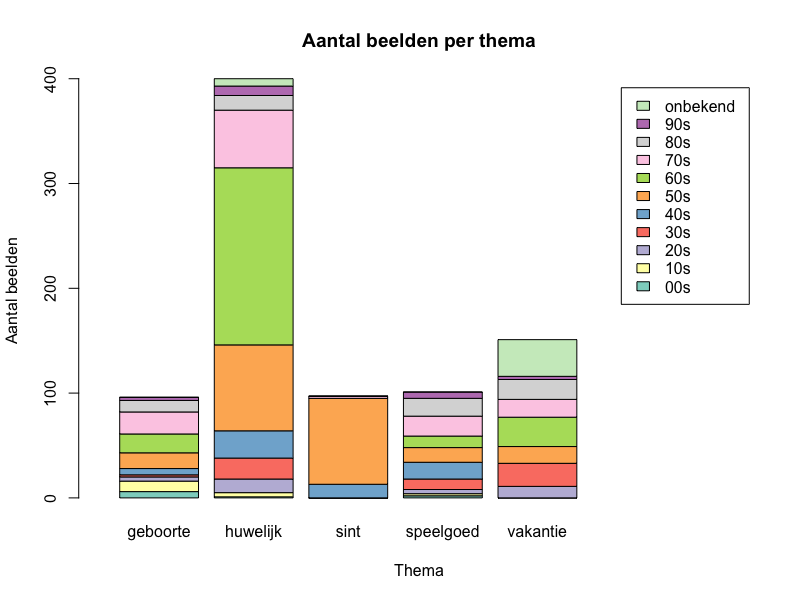
\includegraphics[width=\textwidth]{aantal_beelden_thema.png}\hfill
	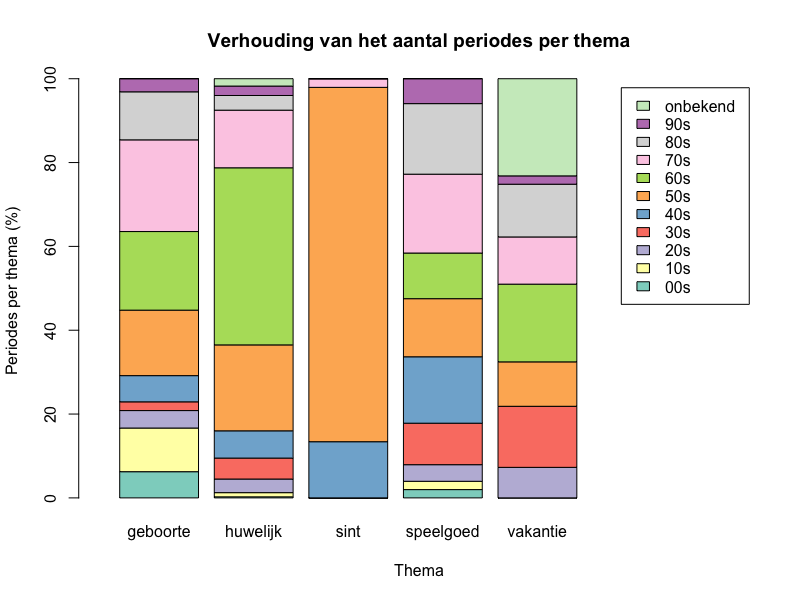
\includegraphics[width=\textwidth]{periode_per_thema.png}\hfill
	\caption[Staafdiagrammen met het aantal beelden per thema en de verhouding van het aantal periodes per thema]{\textbf{Boven:} Het aantal beelden per thema met opsplitsing van de beelden per periode. Het aantal huwelijksfoto's springt er duidelijk uit. \textbf{Onder:} de verhouding van het aantal periodes per thema. Ook hier is het duidelijk dat dit ongelijk verdeeld is.}
\end{figure}


Het valt hierbij op dat de dataset ongelijk verdeeld is:
\begin{itemize}
	%TODO denk aan hoofdletters --> opzoeken
	\item bijna de helft van de dataset bestaat uit huwelijksfoto’s. De andere thema’s zijn meer gelijk verdeeld met grofweg honderd foto’s per thema. 
	\item daarenboven concentreren de huwelijksfoto’s zich op drie periodes. Bijna 75\% van de foto’s zijn afkomstig uit de periode 50s, 60s en 70s. 
	\item de Sinterklaasfoto’s zijn afkomstig uit slechts drie periodes (40s, 50s en 70s) waarvan bijna 85\% uit één periode (50s).
	\item de ongelijke verdeling van de foto’s per thema heeft ook een gevolg op de foto’s per periode. Er zijn vooral foto’s afkomstig uit de periodes 50s, 60s en 70s. Voor 50s gaan bijna 80\% van de foto’s over huwelijk en Sinterklaas, voor de 60s bijna 75\% over huwelijk en voor de 70s zijn 50\% huwelijksfoto’s. Van de vroegste periodes (00s en 10s) zijn dan weer weinig foto’s. 
	\item zowel Sinterklaas- als vakantiefoto’s komen niet in alle periodes voor.
\end{itemize}

Bij het interpreteren van de resultaten moet rekening gehouden worden met deze ongelijke verdeling.

\section{Keuze voor API}
\label{sec:keuze-voor-api}

Clarifai werd als API gekozen om de onderzoeksvraag te beantwoorden. 

Clarifai is gesticht in 2013 door Matthew Zeiler. Hij had in 2013 deelgenomen aan de ImageNet Challenge als doctoraatsstudent samen met zijn promotor Dr. Rob Fergus. Hun architectuur, ZFNet, waarop ook Clarifai gebouwd is, was de winnaar van de ImageNet Challenge~\autocite{Tsang2018}.

De keuze viel op deze API om een aantal redenen:
\begin{enumerate}
	\item De website bevat goede en duidelijke documentatie om met de API aan de slag te gaan. De uitleg wordt telkens voorzien van een voorbeeld in de ondersteunde programmeertalen.
	\item De API heeft clients in verschillende programmeertalen die het de ontwikkelaar mogelijk maken om de API te gebruiken in de programmeertaal naar keuze. JavaScript, Python, Java, C\# en PHP hebben officiële clients die door Clarifai ondersteund en ontwikkeld worden. De REST API kan ook rechtstreeks bevraagd worden zonder gebruikt van een API client~\autocite{ClarifaiAPI}.
	\item De Clarifai website beschikt over een grafische interface waarin gebruikers beelden kunnen opladen om ze te laten taggen door een van de ingebouwde modellen of een nieuw model kunnen trainen. Dit verhoogt het gebruiksgemak, wat, zoals besproken in~\ref{sec:probleemstelling}, een belangrijke factor was bij de keuze voor een API.
	\item Er zijn verschillende ingebouwde modellen die gebruikt kunnen worden om beelden te taggen, gaande van zeer algemene modellen (het general model) tot zeer specifieke modellen, zoals een model om modeconcepten te herkennen of een model om elementen met betrekking tot voeding en vaatwerk te detecteren.
\end{enumerate}

\section{Beelden beschikbaar maken via een publieke URL}
\label{sec:beelden-via-URL}

%TODO uitleggen waarom geen base64
Het Huis van Alijn bracht ons de beelden aan op een harde schijf. De beelden waren immers nog niet online beschikbaar. Om op een geautomatiseerde manier de API van Clarifai te kunnen bevragen, moest een publieke URL voor de beelden voorzien worden. Het waren hoge resolutie beelden waarvan het merendeel in TIFF-formaat was en een kleiner deel in JPEG-formaat. De meeste beelden hadden daarom een bestandsgrootte (10 \'{a} 13 MB per beeld) die te groot is voor Clarifai. Clarifai wil immers beelden met een grootte van maximum 3,6 MB. 

De beelden werden daarom op een beeldenserver geplaatst waarmee met een URL het beeld opgevraagd kon worden in een kleinere bestandsgrootte in het JPEG-bestandsformaat. Clarifai kan immers niet omgaan met beelden groter dan 3,6 MB. Een andere optie was om de beelden te converteren naar JPEG, ze daarbij te verkleinen naar een breedte van 512 pixels en ze vervolgens op een webserver of FTP-server te plaatsen. Clarifai verkleint immers zelf alle beelden tot 512 pixels en hoe dichter je bij dat formaat komt, hoe sneller de API calls verlopen~\autocite{Clairbot2019}. Dit laatste ontdekten we echter pas nadat de test al uitgevoerd was. Het was namelijk niet opgenomen in de documentatie.

De beelden werden opgeladen in een Amazon AWS EC2 Ubuntu instance waarop de beeldenserver (Cantaloupe) ge\"{i}nstalleerd was. Op die manier kreeg ieder beeld een publieke URL die gebruikt kon worden bij het aanroepen van de Clarifai API.

\section{Beschikbare metadata verzamelen in een CSV}
\label{sec:metadata-verzamelen-csv}

De 845 beelden van Huis van Alijn waren voorzien van metadata die uit de bestandsnaam van de digitale bestanden gehaald konden worden. De bestandsnamen hadden volgende logica waarmee het oorspronkelijke medium van het digitale bestand (foto of dia) en het decennium waarin de foto gemaakt was, gehaald kon worden: MEDIUM-DECENNIUM-VOLGNUMMER. Bestanden die startten met \textit{FO} waren digitale kopieën van foto’s, zij die startten met \textit{DIA} van diapositieven. 

Er werd een CSV gecreëerd waarin alle beschikbare metadata per beeld verzameld werden:
\begin{itemize}
	\item base (URL): de URL van het beeld die in vorige stap gecreëerd werd;
	\item bestandsnaam of ID van het beeld;
	\item de extensie of het oorspronkelijke bestandsformaat van het beeld: .tif of .jpg;
	\item type: foto, diapositief of onbekend;
	\item thema;
	\item periode (decennium)
\end{itemize}

%TODO voetnoot toevoegen
Om deze informatie te verzamelen, werd een shell script geschreven. Op de harde schijf waren de afbeeldingen verzameld in een mapje (directory) per thema. Informatie zoals extensie, type, thema en periode werden uit de bestandsnaam gehaald. 

\section{Uitvoeren van workflows}
\label{sec:uitvoeren-workflows}

Er werden twee workflows een aantal keer doorlopen bij het uitvoeren van dit onderzoek:
\begin{itemize}
	\item een workflow om de beelden te laten taggen door Clarifai;
	\item een workflow om via training een custom model te cre\"{e}ren.
\end{itemize}

\subsection{Workflow 1: Een dataset laten taggen door Clarifai}
\label{subsec:workflow1}

\subsubsection{De Clarifai API aanroepen}
\label{(subsubsec:clarifai-aanroepen)}

Clarifai beschikt over API-clients in verschillende programmeertalen (Java, Python, Javascript, C\#, Objective-C en PHP), maar doordat we zelf het meeste voeling hebben met shell scripting, werd gekozen om de REST API te bevragen via cURL, een command-line programma voor het verkrijgen of verzenden van bestanden met behulp van  een URL.

Een API key is nodig om de API te bevragen. Daarom werd eerst een account bij Clarifai aangemaakt. Automatisch verkrijg je dan een gratis key. 

%TODO screenshot van aanmaken van account

Het general model van Clarifai werd gebruikt om de volledige dataset van Huis van Alijn te taggen. Dit is namelijk het meest uitgebreide model met de meeste concepten. het bevat ongeveer 11.000 verschillende concepten waaronder objecten, thema's, emoties in verschillende talen. Daardoor kan het model gebruikt worden voor een reeks van zeer uiteenlopende beelden.{ClarifaiGeneral}

Om via de Clarifai API tags te krijgen voor een beeldbestand via het general model, moet onderstaande commando ingegeven worden in de command line. \$\{API\_key\} en \$\{url\_naar\_het\_beeld\} moeten vervangen worden door respectievelijk de API key en de URL van het beeld. In de URL moet je verwijzen naar de id van het model en de id van de versie van het model die je wenst te gebruiken.~\autocite{ClarifaiAPI}. % TODO voeg het model id en het version id van het general model toe.

\begin{lstlisting}[language=bash,caption=bash commando om een beeld door Clarifai te laten taggen.]
#!/bin/bash
curl -X POST
    -H 'Authorization: Key "${API_key}"'
    -H 'Content-Type: application/json'
    -d '{
        "inputs": [{
            "data": {
                "image": { 
                    "url": "'"${url_naar_het_beeld}"'"
                    }
                }
            }
        ]
    }'
"https://api.clarifai.com/v2/models/${model_id}/versions/${version_id}/outputs"
\end{lstlisting}

Om de API te bevragen, werd een shell script geschreven.\footnote{\url{https://github.com/nvanderperren/bachelorproef/blob/master/research/scripts/predict_image.sh})} Het bevragen van de API verliep vlot. Gemiddeld waren er per beeld twee à drie seconden nodig. Bij drie beelden mislukte het aanroepen omdat ze een te groot bestandsgrootte hadden. Deze beelden werden verkleind waarna de API opnieuw aangeroepen werd.\footnote{voor deze beelden werd een nieuw script geschreven waarin de gewenste grootte en de bestandsnaam van de beelden als parameter meegegeven kan worden: \url{https://github.com/nvanderperren/bachelorproef/blob/master/research/scripts/predict_image_by_size_id.sh}. Er werd gekozen om alles zoveel mogelijk in een script te zetten in functie van hergebruik.}

\subsubsection{Tags van API in een overzicht verzamelen}
\label{subsubsec:tags-verzamelen-overzicht}

Na het bevragen van de Clarifai API werd per beeld een API response in JSON ontvangen met daarin onder meer de tags die aan de beelden gegeven werden.

\begin{lstlisting}[language=json,caption=een ingekorte versie van een ontvangen API response met voorspellingen van Clarifai .]
{
  "status": {
    "code": 10000,
    "description": "Ok",
    "req_id": "7a70efb773234ba9a3eaf219328782b4"
  },
  "outputs": [{
    "id": "94b039d533454d53b01f2d3f825a097e",
    "status": {
      "code": 10000,
      "description": "Ok"
    },
    "created_at": "2019-04-01T16:14:28.886109228Z",
    "model": {
      "id": "aaa03c23b3724a16a56b629203edc62c",
      "name": "general",
      "created_at": "2016-03-09T17:11:39.608845Z",
      "app_id": "main",
      "output_info": {
        "message": "Show output_info with: GET /models/{model_id}/output_info",
        "type": "concept",
        "type_ext": "concept"
      },
      "model_version": {
        "id": "aa7f35c01e0642fda5cf400f543e7c40",
        "created_at": "2018-03-06T21:10:24.454834Z",
        "status": {
       	  "code": 21100,
          "description": "Model trained successfully"
        }
      },
      "display_name": "General"
   	},
    "input": {
      "id": "d74a5f9d8961406eb5a15e9172be9399",
      "data": {
        "image": {
          "url": "http://ec2-18-191-252-182.us-east-2.compute.amazonaws.com:8182/iiif/2/FO-30-00197/full/full/0/default.jpg"
        }
      }
    },
    "data": {
      "concepts": [{
        "id": "ai_l8TKp2h5",
        "name": "people",
        "value": 0.999308,
        "app_id": "main"
      },{
        "id": "ai_bmls4LpL",
        "name": "group",
        "value": 0.9847269,
        "app_id": "main"
      },{
        "id": "ai_sd6DKdXp",
        "name": "group together",
        "value": 0.9833066,
        "app_id": "main"
      },{
        "id": "ai_RQccV41p",
        "name": "woman",
        "value": 0.9795268,
        "app_id": "main"
      },{
        "id": "ai_VPmHr5bm",
        "name": "adult",
        "value": 0.97893196,
        "app_id": "main"
      }]
    }
  }]
}
\end{lstlisting}

De gegevens werden verzameld in een CSV-bestand die geïmporteerd zal worden in Google Sheets. Google Sheets heeft als voordeel dat resultaten eenvoudig gedeeld kunnen worden met de museummedewerkers en bezit bovendien over ingebouwde reken- en queryfuncties die het analyseren van de resultaten vereenvoudigen. Bovendien kan Google Sheets afbeeldingen in een cel tonen via de \texttt{IMAGE}-functie\footnote{Voor meer info over de IMAGE-functie in Google Sheets, zie: \url{https://support.google.com/docs/answer/3093333?hl=en}}. Dit maakt het veel eenvoudiger om de gegevens te valideren.

Om de tags uit de JSON-bestanden te halen werd een shell script geschreven die per beeld de tags en de waarschijnlijkheidsscore uitleest. Het \texttt{paste}-commando\footnote{voor meer info over \texttt{paste}, zie \url{https://linux.die.net/man/1/paste}} werd vervolgens gebruikt om deze CSV samen te voegen met de CSV uit \textit{\ref{sec:metadata-verzamelen-csv} Beschikbare metadata verzamelen in CSV}.

\begin{lstlisting}[language=bash, caption=Met het \texttt{paste}-commando kunnen twee bestanden samengevoegd worden in Bash]
#!/bin/bash
paste -d , "${csv1}" "${csv2}" > "${samengevoegde_csv}"
\end{lstlisting}

%TODO opnemen van eerste regels van CSV?

\subsubsection{Gegevens valideren}
\label{subsubsec:gegevens-valideren}

Om de kwaliteit van de tags te controleren, werd dezelfde methodologie gebruikt als in \textcite{Vanstappen2019}. In het Google Sheets document werd bij ieder tag een checkbox geplaatst die door de validator aangevinkt moest worden als de tag correct was. Dit had als voordeel dat de validatie relatief snel kon gebeuren en dat ook het verwerken van de resultaten eenvoudig was. 

Tijdens het valideren bleek het aanvinken van correcte tags toch niet zo eenvoudig te zijn. Sommige tags vereisten enige interpretatie die moeilijk is zonder de context van het beeld te kennen. Het gaat om tags zoals \textit{happy}, \textit{music} en \textit{love}. Daarvoor konden we ons baseren op de thema’s van de foto’s. We gingen ervan uit dat mensen op huwelijksfoto’s en geboortefoto’s vol liefde waren, en dat zij, net als mensen op vakantie, gelukkig zijn. 

Een andere moeilijkheid was het herkennen of de kinderen op de foto jongens of meisjes waren, of dat we de mensen op de foto konden beschouwen als bejaarde mensen of niet. We zijn bij het corrigeren van deze tags niet te streng geweest. Bij twijfel, wanneer bijvoorbeeld zowel de tags \textit{boy} als \textit{girl} voorkwamen, hebben we steeds de term met de grootste waarschijnlijkheidsscore goedgekeurd.

Ten slotte waren er ook nog de tags \textit{group}, \textit{several} en \textit{many}. We beschouwden iets een groep als er drie of meer mensen op de foto stonden. De andere tags werden gevoelsmatig goed- of afgekeurd.

\begin{figure}
	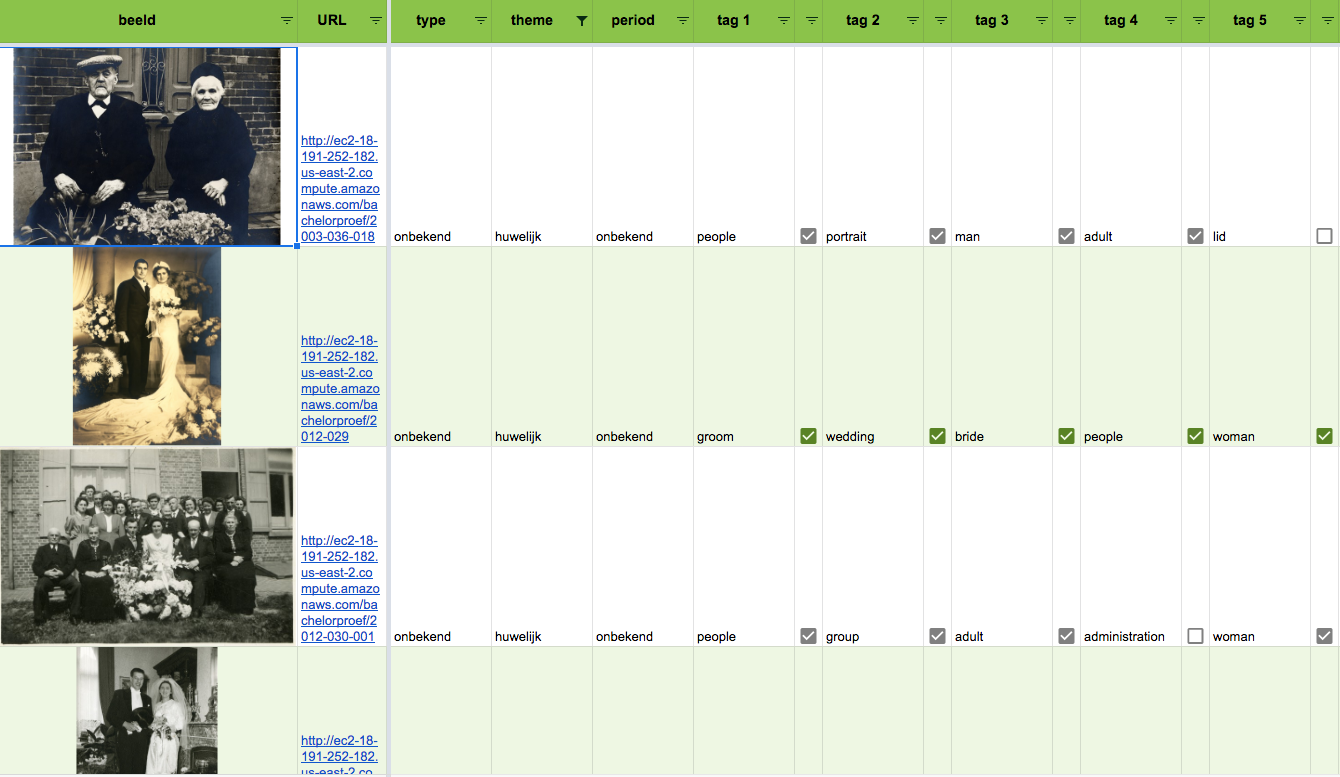
\includegraphics[width=\textwidth]
	{validatiescherm.png}
	\caption{Screenshot van de Google Sheet waarin de validatie plaatsvond.}
	\label{fig:validatiescherm}
\end{figure}

\subsection{Workflow 2: Een custom model trainen}
\label{subsec:workflow2}

Voor het trainen van de API door de creatie van een custom model werd de workflow gevolgd van \textcite{ClarifaiAPI}. Voor dit onderzoek werden twee custom models gemaakt:
\begin{itemize}
	\item een model die de beelden van Huis van Alijn kan classificeren volgens hun thema (geboorte, huwelijk, Sinterklaas, speeldgoed en vakantie), vanaf nu het themamodel;
	\item een model die de beelden van Huis van Alijn kan classificeren volgens het decennium waarin de foto getrokken was (1900s t.e.m. 1990s), vanaf nu het periodemodel.
\end{itemize}

Voor ieder model werden een aantal stappen doorlopen:
\begin{enumerate}
	\item het maken van een trainingsset en validatieset;
	\item het opladen van de trainingsbeelden naar Clarifai;
	\item het creëren van een custom model met de concepten uit de trainingsbeelden;
	\item het trainen van het model;
	\item het valideren van het model met de validatieset.
\end{enumerate}

De getrainde modellen werd vervolgens gebruikte om de hele dataset van Huis van Alijn te classificeren in respectievelijk thema en periode. 

Het is in Clarifai mogelijk om een custom model te maken via de API of via een webinterface. Voor dit onderzoek hebben we gebruik gemaakt van de API.

\subsubsection{Training- en validatieset maken}

Uit de dataset van Huis van Alijn werd een trainingset en een validatieset gemaakt. De trainingsbeelden dienden om het model te trainen; de validatiebeelden om de verschillende iteraties van het model te valideren en te beoordelen welke iteratie het meest performant is~\autocites{Lievens2017}{Brownlee2017}. Door de kleine dataset (845 beelden) wilden we slechts 50\% van de beelden gebruiken voor training; 20\% werd gebruikt als validatieset.

%TODO literatuur invoegen + belang validatieset

Trainingsbeelden en validatiebeelden werden willekeurig geselecteerd uit de dataset. \textcite{Gong2017} meldt dat het erg belangrijk is dat de trainingsbeelden overeenkomen met de beelden waarop het model toegepast zal worden. Er werd daarom gezorgd dat, in de mate van het mogelijke, in de beelden voor respectievelijk het themamodel en het periodemodel alle decennia en thema’s (gelijkmatig) aanwezig waren. Omdat een huwelijk in de jaren 1900 er nu eenmaal anders uitziet dan dat in de jaren 1950 of 1990 is het immers belangrijk dat het model zoveel mogelijk beelden te zien krijgt van hoe een huwelijk eruit kan zien doorheen alle periodes. Het periodemodel moet dan weer weten dat een foto uit een bepaald decennium kan bestaan uit zowel huwelijks-, geboorte-, Sinterklaas-, speelgoed- als vakantiefoto’s.

Voor het themamodel wilden we ieder thema evenwaardig trainen en dus evenveel trainingsbeelden per thema gebruiken. Doordat het aantal beelden per thema ongelijk verdeeld is (vierhonderd huwelijksfoto’s, $\pm$ honderd beelden voor de andere thema’s, zie tabel \ref{tab:analyse-dataset}), beslisten we om het aantal foto’s per thema te beperken tot honderd. Dit hield in dat voor ieder thema slechts vijftig foto’s gebruikt zouden worden als trainingsbeelden en dat de validatieset uit twintig foto’s per thema bestaat. 

Bij het periodemodel was het niet mogelijk om iedere periode evenwaardig te trainen. Het aantal beelden per decennium was hiervoor te ongelijk verdeeld (zie figuur \ref{fig:aantal-beelden-periode}). Er waren bijvoorbeeld minder dan dertig foto’s voor de jaren 00, 10 en 90, en meer dan tweehonderd foto’s voor de jaren 50 en 60. Beperken van het aantal foto’s per periode was daardoor onmogelijk. De trainingset zou dan  te marginaal zijn.

\begin{figure}
	\centering
	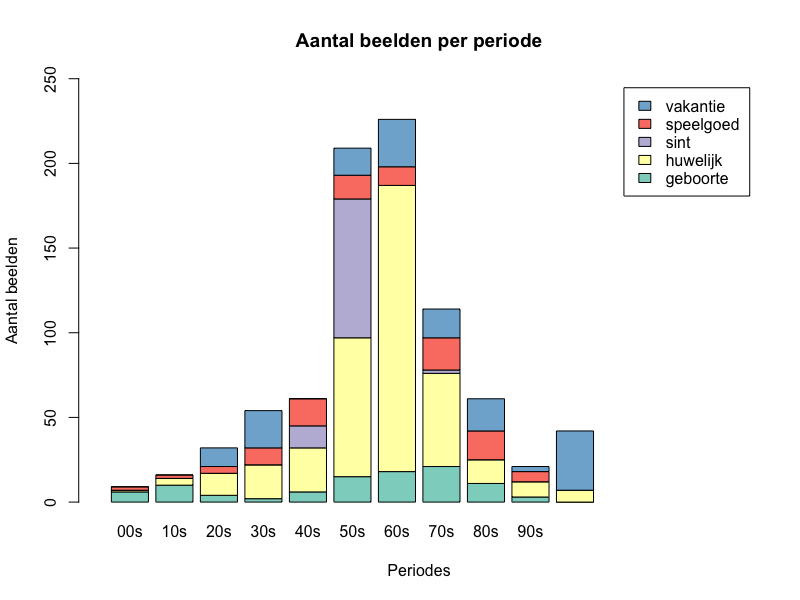
\includegraphics[width=\textwidth]{aantal_beelden_periode.png}\hfill
	\caption[Staafdiagram met het aantal beelden per periode]{Staafdiagram die het aantal beelden per periode weergeeft. De meest rechtse staaf toont het aantal beelden waarvan de periode niet gekend is.}
	\label{fig:aantal-beelden-periode}
\end{figure}


\subsubsection{Trainingsbeelden opladen naar de computer vision service}
\label{subsubsec:trainingsbeelden-opladen}

Om een model te maken, moeten eerst trainingsbeelden opgeladen worden die reeds het concept bevatten waarvan we willen dat het model het herkent~\autocite{ClarifaiAPI}. 

We beslisten om het model in iteraties te trainen. \textcite{ClarifaiAPI} stelt immers voor om te starten met tien beelden per concept en vervolgens meer beelden per concept toe te voegen indien dit nodig blijkt. Na iedere iteratie werd het model gevalideerd. Voor het themamodel werd gewerkt in iteraties van tien trainingsfoto’s per thema. Voor het periodemodel werd dit opgetrokken tot iteraties van maximum dertig trainigsfoto’s per periode\footnote{Waar mogelijk, voor de decennia 00s, 10s, 20s, 30s en 90s waren geen dertig trainingsbeelden beschikbaar.}, omdat het periodemodel een grotere variëteit aan beelden moet herkennen.

%TODO tabel van de iteraties thema

%TODO tabel van de iteraties periode


\begin{lstlisting}[language=bash,caption=bash commando om een beeld met een concept naar Clarifai op te laden.]
#!/bin/bash
curl -X POST \
  -H 'Authorization: Key "${API_key}"' \
  -H 'Content-Type: application/json' \
  -d '{
    "inputs": [{
      "data": {
        "image": {
          "url": "'"${url_naar_het_beeld}"'"
        },
        "concepts":[{
          "id": "'"${concept}"'",
          "value": true
        }]
      }
    }]
  }'\
https://api.clarifai.com/v2/inputs
\end{lstlisting}

\begin{lstlisting}[language=json,caption=Het antwoord van de Computer Vision API in JSON na het opladen van een beeld met een concept]
{
  "status": {
    "code": 10000,
    "description": "Ok",
    "req_id": "f8db86f0ff564086a6611c7dd34e91e3"
  },
  "inputs": [{
    "id": "153005f7c8b04d949356dc36c1bbbee9",
    "data": {
      "image": {
        "url": "http://ec2-18-191-252-182.us-east-2.compute.amazonaws.com:8182/iiif/2/2003-036-018/full/922,/0/default.jpg"
      },
      "concepts": [{
        "id": "huwelijk",
        "name": "huwelijk",
        "value": 1,
        "app_id": "1b9b01460b944923a9eb1578668d4ea6"
      }]
    },
    "created_at": "2019-07-13T13:57:15.569447471Z",
    "modified_at": "2019-07-13T13:57:16.399324215Z",
    "status": {
      "code": 30000,
      "description": "Download complete"
    }
  }]
}
\end{lstlisting}

Het is in Clarifai ook mogelijk om negatieve concepten toe te voegen. Dit zijn concepten die niet op de foto te zien zijn. Op een huwelijksfoto kan bijvoorbeeld aangeduid worden dat dit geen speelgoed-, vakantie-, geboorte- en Sinterklaasfoto is. Om te testen of negatieve concepten een invloed hebben op de resultaten van de validatieset, werd na de eerste iteratie voor alle trainingsbeelden alle negatieve concepten toegevoegd.

\subsubsection{Het model maken}
\label{subsubsec:model-maken}

Nadat de beelden van de eerste iteratie opgeladen werden naar Clarifai, kan het  het model aangemaakt worden. Aan het model moet een naam worden gegeven en de concepten toegevoegd die op de trainingsbeelden te zien zijn. 

Daarnaast kan het model nog geconfigureerd worden. In onze modellen werd ingesteld dat op een beeld slechts één concept bevat\footnote{Een huwelijksfoto kan bijvoorbeeld nooit een vakantiefoto zijn.} (parameter \texttt{concepts\_mutually\_exclusive}) en dat er geen gebruik gemaakt wordt van trainingsbeelden waarop geen enkel concepten te zien is (parameter \texttt{closed\_environment})

\begin{lstlisting}[language=bash,caption=bash commando om een custom model met vijf concepten te creëren]
#!/bin/bash
curl -X POST \
  -H 'Authorization: Key "${API_key}"' \
  -H 'Content-Type: application/json' \
  -d '{
    "model": {
      "id": "HvA_theme",
      "output_info": {
        "data": {
          "concepts": [{
            "id": "'"${concept1}"'"
          },{
            "id": "'"${concept2}"'"
          },{
            "id": "'"${concept3}"'"
          },{
            "id": "'"${concept4}"'"
          },{
            "id": "'"${concept5}"'"
          }]
        },
        "output_config": {
          "concepts_mutually_exclusive": true,
          "closed_environment": true
        }
      }
    }
  }'\
  https://api.clarifai.com/v2/models
\end{lstlisting}

\begin{lstlisting}[language=json,caption=antwoord van de API na het creëren van het model]
{
  "status": {
    "code": 10000,
    "description": "Ok",
    "req_id": "66be8c1a7bbc4cca9398d02c7c15a097"
  },
  "model": {
    "id": "HvA_theme",
    "name": "HvA_theme",
    "created_at": "2019-07-13T14:15:49.966900528Z",
    "app_id": "1b9b01460b944923a9eb1578668d4ea6",
    "output_info": {
      "output_config": {
        "concepts_mutually_exclusive": true,
        "closed_environment": true,
        "max_concepts": 0,
        "min_value": 0,
        "test_split_percent": 10
      },
      "message": "Show output_info with: GET /models/{model_id}/output_info",
      "type": "concept",
      "type_ext": "concept"
    },
    "model_version": {
      "id": "68b9e3c20ae04abbbdc2e3fb974b9a0f",
      "created_at": "2019-07-13T14:15:49.994520471Z",
      "status": {
        "code": 21102,
        "description": "Model not yet trained"
      },
      "active_concept_count": 5
    }
  }
}
\end{lstlisting}

\subsubsection{Het model trainen}
\label{subsubsec:model-trainen}

Telkens er nieuwe trainingsbeelden toegevoegd zijn, moet het model getraind worden. Door het trainen van het model gaat het systeem naar alle beelden met de concepten kijken en daarvan leren~\autocite{ClarifaiAPI}. 


\begin{lstlisting}[language=bash,caption=bash commando om het model te trainen]
#!/bin/bash
curl -X POST \
  -H 'Authorization: Key "${API_key}"' \
  -H 'Content-Type: application/json' \
  "https://api.clarifai.com/v2/models/${model_id}/versions" 
\end{lstlisting}

\begin{lstlisting}[language=json,caption=antwoord van de API nadat het model getraind werd]
{
  "status": {
    "code": 10000,
    "description": "Ok",
    "req_id": "2f513295f4074ec39115e3e5e500d652"
  },
  "model": {
    "id": "HvA_theme",
    "name": "HvA_theme",
    "created_at": "2019-07-13T14:15:49.966900Z",
    "app_id": "1b9b01460b944923a9eb1578668d4ea6",
    "output_info": {
      "output_config": {
        "concepts_mutually_exclusive": true,
        "closed_environment": true,
        "max_concepts": 0,
        "min_value": 0,
        "test_split_percent": 10
      },
      "message": "Show output_info with: GET /models/{model_id}/output_info",
      "type": "concept",
      "type_ext": "concept"
    },
    "model_version": {
      "id": "b6fd2a1befd947bdb200b5e635721657",
      "created_at": "2019-07-13T14:28:25.060240688Z",
      "status": {
        "code": 21103,
         "description": "Custom model is currently in queue for training, waiting on inputs to process."
      },
      "active_concept_count": 5
    }
  }
}
\end{lstlisting}

Na het trainen krijgt het model een versiecode. Met deze code is het mogelijk om bij het voorspellen een bepaalde versie van het model te gebruiken. Als blijkt dat het model na iteratie 3 beter is dan dat van iteratie 4, dan kan je met de versiecode het model van iteratie 3 gebruiken.

\subsubsection{Het model valideren}
\label{subsubsec:model-valideren}

Nadat het model getraind was, werd het uitgetest op de validatieset. Hiervoor werd workflow 1 uit \ref{subsec:workflow1} doorlopen met de validatiesets voor de twee modellen.

Om het model te beoordelen werd gebruik gemaakt van de gemiddelde rappel, precisie en \textit{F}-score~\autocite{Lievens2017}:
\begin{itemize}
    \item De rappel is het percentage van de positieve trainingsbeelden die ook effectief als positief werd gelabeld door het model (verhouding tussen het aantal true positives en het totaal aantal positieve voorbeelden van het concept);
    \item De precisie is het percentage van de beelden die als een bepaald concept herkend werken daadwerkelijk dat concept bevatten (verhouding tussen het aantal true positives en het totaal aantal herkende beelden voor dat concept);
    \item De precisie en de rappel kunnen gecombineerd worden in één enkele score, de \textit{F}-score. Om een grote \textit{F}-score te behalen moeten zowel de precisie als de rappel het goed doen.
\end{itemize}

Hoe groter deze scores, hoe performanter het model. Clarifai geeft meerdere concepten aan een model. Er werd enkel rekening gehouden met het concept dat de hoogste waarschijnlijkheidsscore gekregen heeft. Hierbij werd geen drempelwaarde ingesteld. Dit betekent dat als aan een beeld een correct concept toegekend werd met een waarschijnlijkheid van 10\%, dat deze ook als een true positive bestempeld werd. 

De hoogste \textit{F}-score voor het Themamodel werd behaald in de vierde iteratie met een score van 92\% (tabel \ref{tab:validatie-themamodel}). In de vijfde iteratie daalt de score licht tot 91\%. Na de eerste iteratie (tien trainingsbeelden voor ieder thema) werd er al een \textit{F}-score van 78\% behaald. Het toevoegen van veertig negatieve voorbeelden na de eerste iteratie zorgde voor een lichte stijging tot 80\%. Als de vierde iteratie van naderbij bekeken wordt (tabel \ref{tab:validatie-iteratie4-themamodel}), dan valt het op dat het model erg goed is in het classificeren van de Sinterklaasfoto’s (score van 100\%). Het minst scoorde op de speelgoed- en geboortefoto’s met een \textit{F}-score van respectievelijk 84\% en 85\%. Bij de speelgoedfoto’s werd een lagere rappel behaald (80\%), maar was de precisie hoger (89\%). 

\begin{table}
    \centering
    \begin{tabular}{l|cc|c}
        \toprule
        & aantal positieven  &  aantal negatieven & \textit{F}-score (\%)\\
        \midrule
        iteratie 1/A & 10 & 0 & 78 \\
        iteratie 1/B & 10 & 40 & 80 \\
        iteratie 2 & 20 & 40 & 86 \\
        iteratie 3 & 30 & 40 & 88 \\
        iteratie 4 & 40 & 40 & 92 \\
        iteratie 5 & 50 & 40 & 91 \\
        \bottomrule
    \end{tabular}
    \caption[De \textit{F}-scores voor de verschillende iteraties van het Themamodel.]{De \textit{F}-scores voor de verschillende iteraties van het Themamodel met vermelding van het aantal postieve en negatieve voorbeelden per thema na iedere iteratie.}
    \label{tab:validatie-themamodel}
\end{table}


\begin{table}
    
    \begin{tabular}{l|ccc|rrr}
        \toprule
        & true positives  & false negatives & false positives & rappel & precisie & \textit{F}-score \\
        \midrule
        geboorte & 17 & 3 & 3 & 85\% & 85\% & 85\% \\
        huwelijk & 20 & 0 & 2 & 100\% & 91\% & 95\% \\
        Sint & 20 & 0 & 0 & 100\% & 100\% & 100\% \\
        speelgoed & 16 & 4 & 2 & 80\% & 88,9\% & 84,2\% \\
        vakantie & 19 & 1 & 1 & 95\% & 95\% & 95\% \\
        \midrule
        gemiddelde & 18,4 & 1,6 & 1,6 & 92\% & 92\% & 91,9\% \\
        \bottomrule
    \end{tabular}
    \caption{De resultaten (rappel, precisie en \textit{F}-score) van de vierde iteratie bij het trainen van het Themamodel.}
    \label{tab:validatie-iteratie4-themamodel}
\end{table}

Bij het Periodemodel, met de onevenwichtige en beperkte trainingset, werd op de validatieset slechtst een maximale \textit{F}-score van 48\% behaald na iteratie 2. Het valt op dat vanaf iteratie 3 de score weer daalt. Een mogelijke verklaring is dat het aantal trainingsbeelden per periode te verschillend is. De rappel en de precisie stijgen voor een beperkt aantal periodes, maar dalen voor alle andere periodes. Het toevoegen van negatieve voorbeelden na iteratie 1 brengt geen verandering in de rappel, precisie en \textit{F}-score. Iteratie 1 en iteratie 1 met negatieven hebben beiden een F-score van 40\%. Iteratie 2 behaalde de grootste rappel voor beelden uit de jaren 40 (67\%) en de grootste precisie op beelden uit de jaren 10 (100\%). De grootste globale score werd behaald op beelden uit de jaren 80 met een F-score van 58\%. Het model scoorde het slechtst op foto’s uit het eerste decennium de jaren 1900 en de jaren 90, met een \textit{F}-score van respectievelijk 0\% en 29\%. Dit zijn periodes met weinig trainingsbeelden (resectievelijk vier en tien). Het is opmerkelijk dat het model bij foto's van de jaren 10 toch een \textit{F}-score van 50\% behaalt, terwijl deze periode ook maar acht trainingsbeelden heeft.

\begin{table}
	\centering
	\begin{tabular}{l|cc|c}
		\toprule
		& aantal positieven  &  aantal negatieven &  \textit{F}-score (\%)\\
		\midrule
		iteratie 1/A & 21,5 & 0 & 39,9 \\
		iteratie 1/B & 21,5 & 193,5 & 39,9 \\
		iteratie 2 & 30,2 & 193,5 & 48 \\
		iteratie 3 & 36,2 & 193,5 & 47,3 \\
		iteratie 4 & 39,9 & 193,5 & 43,9 \\
		\bottomrule
	\end{tabular}
	\caption[De \textit{F}-scores voor de verschillende iteraties van het Periodemodel.]{De \textit{F}-scores voor de verschillende iteraties van het Periodemodel met vermelding van het gemiddeld aantal postieve en negatieve voorbeelden per thema na iedere iteratie. Zie figuur om een beeld te hebben van de volledige spreiding van de trainingset}
	\label{tab:validatie-periodemodel}
\end{table}

\begin{table}
	\begin{tabular}{l|ccc|rrr}
		\toprule
		& true positives  & false negatives & false positives & rappel & precisie & \textit{F}-score \\ 
		\midrule
		00s & 0 & 2 & 0 & 0\% & 0\% & 0\% \\ 
		10s & 1 & 2 & 0 &  33\% & 100\% & 50\% \\ 
		20s & 4 & 3 & 5 & 57\% & 44,4\% & 50\% \\ 
		30s & 5 & 5 & 12 & 50\% & 29,4\% & 37\% \\ 
		40s & 8 & 4 & 13  & 67\% & 38,1\% & 48,5\% \\ 
		50s & 15 & 23 & 15  & 39\% & 50\% & 44\% \\ 
		60s & 13 & 21 & 13  & 48\% & 59,4\% & 52,8\% \\ 
		70s & 12 & 9 & 12  & 55\% & 47,8\% & 51,2\% \\ 
		80s & 5 & 5 & 5  & 58\% & 58,3\% & 58,3\% \\ 
		90s & 2 & 3 & 2  & 25\% & 33,3\% & 28,6\% \\ 
		\midrule
		gemiddelde & 7,1 & 7,7 & 7,7  & 43\% & 46,1\% & 42,1\% \\ 
		\bottomrule
	\end{tabular} 
	\caption{De resultaten (rappel, precisie en \textit{$F_{1}$}-score) van de tweede iteratie bij het trainen van het Periodemodel.}
	\label{tab:validatie-iteratie2-periodemodel}
\end{table}

Wat doet de scores dalen na een hogere iteratie? Bij het Periodemodel vermoedden we dat dit komt door het onevenwicht in het aantal trainingsbeelden tussen de verschillende periodes, maar voor het Themamodel is dit moeilijker te bepalen omdat de thema’s even goed getraind zijn. Misschien komt het door een licht onevenwicht in het aantal periodes in de trainingsbeelden van het themamodel? Bij iteratie 4 liggen de aantallen iets dichter op mekaar (met een uitschieter voor de jaren 50), terwijl in iteratie 5 de uitschieter van de jaren 50 nog groter geworden is. Ook bij het periodemodel zien we de verhouding tussen het aantal thema’s in de foto’s groter worden na iteratie 2. Dit moet verder onderzocht worden met grotere datasets om hier conclusies uit te trekken. Een andere mogelijkheid is dat we op de grenzen van de CV API gestoten zijn.
